\documentclass[portrait,final,a0paper]{baposter}
%\documentclass[a4shrink,portrait,final]{baposter}
% Usa a4shrink for an a4 sized paper.

\tracingstats=2

\usepackage{calc}
\usepackage{graphicx}
\usepackage{amsmath}
\usepackage{amssymb}
\usepackage{relsize}
\usepackage{multirow}
\usepackage{bm}

\usepackage{graphicx}
\usepackage{multicol}

\usepackage{pgfbaselayers}
\pgfdeclarelayer{background}
\pgfdeclarelayer{foreground}
\pgfsetlayers{background,main,foreground}

\usepackage{times}
\usepackage{helvet}
%\usepackage{bookman}
\usepackage{palatino}

\newcommand{\captionfont}{\footnotesize}

\selectcolormodel{cmyk}

\graphicspath{{images/}}

%%%%%%%%%%%%%%%%%%%%%%%%%%%%%%%%%%%%%%%%%%%%%%%%%%%%%%%%%%%%%%%%%%%%%%%%%%%%%%%%
%%%% Some math symbols used in the text
%%%%%%%%%%%%%%%%%%%%%%%%%%%%%%%%%%%%%%%%%%%%%%%%%%%%%%%%%%%%%%%%%%%%%%%%%%%%%%%%
% Format 
\newcommand{\Matrix}[1]{\begin{bmatrix} #1 \end{bmatrix}}
\newcommand{\Vector}[1]{\Matrix{#1}}
\newcommand*{\SET}[1]  {\ensuremath{\mathcal{#1}}}
\newcommand*{\MAT}[1]  {\ensuremath{\mathbf{#1}}}
\newcommand*{\VEC}[1]  {\ensuremath{\bm{#1}}}
\newcommand*{\CONST}[1]{\ensuremath{\mathit{#1}}}
\newcommand*{\norm}[1]{\mathopen\| #1 \mathclose\|}% use instead of $\|x\|$
\newcommand*{\abs}[1]{\mathopen| #1 \mathclose|}% use instead of $\|x\|$
\newcommand*{\absLR}[1]{\left| #1 \right|}% use instead of $\|x\|$

\def\norm#1{\mathopen\| #1 \mathclose\|}% use instead of $\|x\|$
\newcommand{\normLR}[1]{\left\| #1 \right\|}% use instead of $\|x\|$

\def\bi{\begin{itemize}}
\def\ei{\end{itemize}}
\def\im{\item}

%%%%%%%%%%%%%%%%%%%%%%%%%%%%%%%%%%%%%%%%%%%%%%%%%%%%%%%%%%%%%%%%%%%%%%%%%%%%%%%%
% Multicol Settings
%%%%%%%%%%%%%%%%%%%%%%%%%%%%%%%%%%%%%%%%%%%%%%%%%%%%%%%%%%%%%%%%%%%%%%%%%%%%%%%%
\setlength{\columnsep}{0.7em}
\setlength{\columnseprule}{0mm}


%%%%%%%%%%%%%%%%%%%%%%%%%%%%%%%%%%%%%%%%%%%%%%%%%%%%%%%%%%%%%%%%%%%%%%%%%%%%%%%%
% Save space in lists. Use this after the opening of the list
%%%%%%%%%%%%%%%%%%%%%%%%%%%%%%%%%%%%%%%%%%%%%%%%%%%%%%%%%%%%%%%%%%%%%%%%%%%%%%%%
\newcommand{\compresslist}{%
\setlength{\itemsep}{1pt}%
\setlength{\parskip}{0pt}%
\setlength{\parsep}{0pt}%
}


%%%%%%%%%%%%%%%%%%%%%%%%%%%%%%%%%%%%%%%%%%%%%%%%%%%%%%%%%%%%%%%%%%%%%%%%%%%%%%
%%% Begin of Document
%%%%%%%%%%%%%%%%%%%%%%%%%%%%%%%%%%%%%%%%%%%%%%%%%%%%%%%%%%%%%%%%%%%%%%%%%%%%%%

\begin{document}

%%%%%%%%%%%%%%%%%%%%%%%%%%%%%%%%%%%%%%%%%%%%%%%%%%%%%%%%%%%%%%%%%%%%%%%%%%%%%%
%%% Here starts the poster
%%%---------------------------------------------------------------------------
%%% Format it to your taste with the options
%%%%%%%%%%%%%%%%%%%%%%%%%%%%%%%%%%%%%%%%%%%%%%%%%%%%%%%%%%%%%%%%%%%%%%%%%%%%%%
% Define some colors

\definecolor{yellow}{cmyk}{0,0,0.9,0.0}
\definecolor{reddishyellow}{cmyk}{0,0.22,1.0,0.0}
\definecolor{black}{cmyk}{0,0,0.0,1.0}
\definecolor{darkYellow}{cmyk}{0,0,1.0,0.5}
\definecolor{lightyellow}{cmyk}{0,0,0.3,0.0}
\definecolor{lighteryellow}{cmyk}{0,0,0.1,0.0}
\definecolor{lighteryellow}{cmyk}{0,0,0.1,0.0}
\definecolor{lightestyellow}{cmyk}{0,0,0.05,0.0}

\definecolor{silver}{cmyk}{0,0,0,0.3}
\definecolor{lightsilver}{cmyk}{0,0,0,0.15}
\definecolor{lightersilver}{cmyk}{0,0,0,0.10}
\definecolor{lightestsilver}{cmyk}{0,0,0,0.01}
\definecolor{darkSilver}{cmyk}{0,0,0,0.1}
\definecolor{white}{cmyk}{0,0,0,0}

\definecolor{h-alpha}{cmyk}{0,0.74,0.34,0.35}
\definecolor{h-alpha-2}{cmyk}{0,0.05,0.02,0.17}
\definecolor{dark_red_1}{rgb}{1, 0.1,0.1}
\definecolor{dark_red_2}{rgb}{0.8, 0.2,0.2}
\definecolor{darkblue}{cmyk}{0.93,0.93,0,0.78}
\definecolor{blue}{cmyk}{0.53,0.53,0,0.62}

%%
\typeout{Poster Starts}
\background{
  \begin{tikzpicture}[remember picture,overlay]%
    \draw (current page.north west)+(-2em,2em) node[anchor=north west] {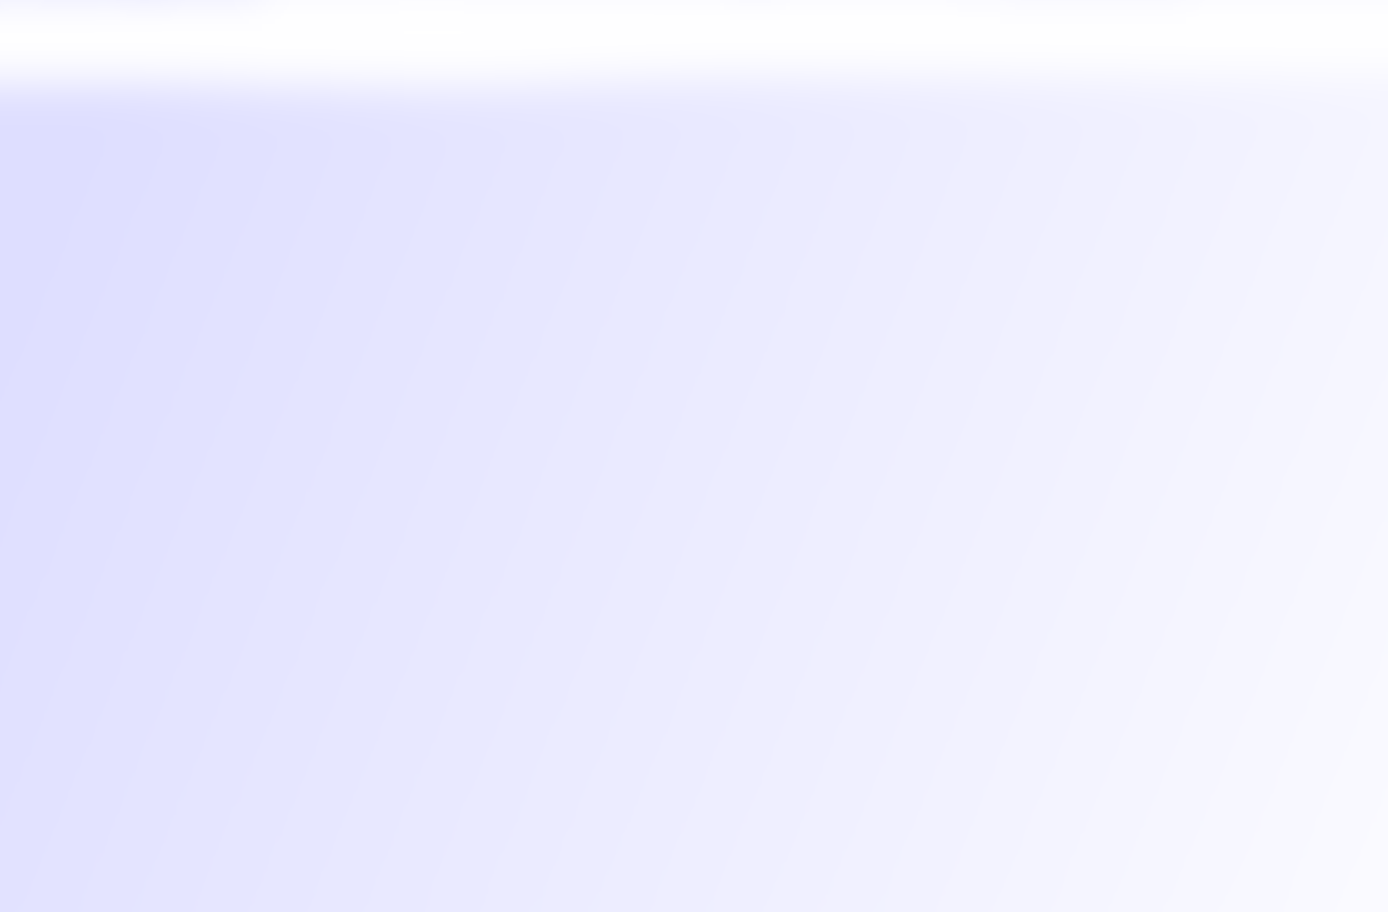
\includegraphics[height=1.1\textheight]{silhouettes_background}};
  \end{tikzpicture}%
}

\newlength{\leftimgwidth}
\begin{poster}%
  % Poster Options
  {
  % Show grid to help with alignment
  grid=no,
  % Column spacing
  colspacing=1em,
 % ============Ondra G pokus o H aplha ==============
  bgColorOne=white,  %First background color. There are two background color to allow for background gradients.
  %bgColorTwo=lightestsilver,
  borderColor=h-alpha-2,		%Color used for the borders of the poster boxes
  headerColorTwo=darkblue,	%First color of box header. Two colors can be used to dene gradients.
  headerColorOne=blue,
  headerFontColor=white,
  boxColorOne=h-alpha-2,
  boxColorTwo=white,
%=========== barevné přechody==========
 % Format of textbox
% ==========nové ===============
  textborder=roundedleft,  %Which kind of border should the lower part of the text boxes have. Possible values are:
			    %1. none 2. bars 3. coils 4. triangles 5. rectangle 6. rounded 7. faded
  % Format of text header
  headerborder=open,%At which sides of the text box headers should we draw a border. Possible values are:
		    %1. none 2. closed 3. open
  headershape=roundedright,
  headershade=shade-tb, %1. plain 2. shade-lr 3. shade-tb 4. shade-tb-inverse
  boxshade=shade-lr,
  background=plain,
% % Color style
%  ============žlutá ==============
%   bgColorOne=lighteryellow,
%   bgColorTwo=lightestyellow,
%   borderColor=reddishyellow,
%   headerColorOne=yellow,
%   headerColorTwo=reddishyellow,
%   headerFontColor=black,
%   boxColorOne=lightyellow,
%   boxColorTwo=lighteryellow,
% ============stříbrná ==============
  %bgColorOne=lightersilver,  %First background color. There are two background color to allow for background gradients.
  %bgColorTwo=lightestsilver,
  %borderColor=silver,		%Color used for the borders of the poster boxes
  %headerColorOne=silver,	%First color of box header. Two colors can be used to dene gradients.
  %headerColorTwo=lightersilver,
  %headerFontColor=black,
  %boxColorOne=lightestsilver,
  %boxColorTwo=white,
%=%========== barevné přechody==========
 % Format of textbox
% ==========nové ===============
%  textborder=roundedleft,  %Which kind of border should the lower part of the text boxes have. Possible values are:
%			    %1. none 2. bars 3. coils 4. triangles 5. rectangle 6. rounded 7. faded
%  % Format of text header
%  headerborder=open,%At which sides of the text box headers should we draw a border. Possible values are:
%		    %1. none 2. closed 3. open
%  headershape=roundedright,
%  headershade=shade-tb, %1. plain 2. shade-lr 3. shade-tb 4. shade-tb-inverse
%  boxshade=shade-lr,
%  background=shade-tb,
%==========původní ===============
%   % Format of textbox
%   textborder=roundedleft,
%   % Format of text header
%   headerborder=open,
%   headershape=roundedright,
%   headershade=plain,
%   boxshade=plain,
%   background=plain,
% zbytek
  headerfont=\Large\textsf, %Sans Serif
  headerheight=0.12\textheight,%Height of the main poster header (not of the headers of the text boxes).
  eyecatcher=yes,
  linewidth=2pt
  }
  % Eye Catcher
  {
\includegraphics[width=7em]{golem.pdf}} % No eye catcher for this poster. (eyecatcher=no above). If an eye catcher is present, the title is centered between eye-catcher and logo.
  % Title
  {%\sf %Sans Serif
  \sc\huge Electron Density Measurement at the GOLEM Tokamak \vspace{ 0.2cm}}
  % Authors
  {Ondřej Grover
  %Sans Serif
  % Serif
  %E. Bromov\'a$^1$, I. \v Duran$^2$, O. Grover$^1$, J. Kocman$^1$, T. Markovi\v{c}$^1$, M. Odstr\v cil$^{12}$, T.\,Odstr\v cil$^1$\!, O.\,Pluha\v r$^3$\!, J.\,St\" ockel$^2$\!, V.\,Svoboda$^1$\!, A.\,\v Sindlery$^1$\!, G.\,Vondr\'a\v sek$^1$\!, J.\,Zara$^3$\!.\\
%{\large $^1$Faculty of Nuclear Sciences and Physical Engineering CTU Prague, CZ-115 19, Czech Rep.\\$^2$Institute of Plasma Physics AS CR, CZ-182 21 Prague, Czech Republic.\\$^3$Faculty of Electrical Engineering CTU Prague, CZ-166 27, Czech Rep.}
}{
    \makebox[8em][r]{%
      \begin{minipage}{8em}
	
\includegraphics[width=7em]{lev}
      %  
\includegraphics[width=7em]{logoipp}
      \end{minipage}}
}


%%%%%%%%%%%%%%%%%%%%%%%%%%%%%%%%%%%%%%%%%%%%%%%%%%%%%%%%%%%%%%%%%%%%%%%%%%%%%%
%%% Now define the boxes that make up the poster
%%%---------------------------------------------------------------------------
%%% Each box has a name and can be placed absolutely or relatively.
%%% The only inconvenience is that you can only specify a relative position 
%%% towards an already declared box. So if you have a box attached to the 
%%% bottom, one to the top and a third one which should be in between, you 
%%% have to specify the top and bottom boxes before you specify the middle 
%%% box.
%%%%%%%%%%%%%%%%%%%%%%%%%%%%%%%%%%%%%%%%%%%%%%%%%%%%%%%%%%%%%%%%%%%%%%%%%%%%%%
%%%%%%%%%%%%%%%%%%%%%%%%%%%%%%%%%%%%%%%%%%%%%%%%%%%%%%%%%%%%%%%%%%%%%%%%%%%%%%
\headerbox{Introduction}{name=intro,column=0,row=0}
{
Electron density measurement is one of the standard diagnostics in the field of plasma physics. Since 2007 when the device back then named CASTOR was transfered to the Faculty of Nuclear Physics and Engineering from the Czech Academy of Sciences, several original and also new diagnostics have been implemented. 

The goals of this project were to implement the standard line-averaged electron density measurement via microwave interferometry. This consisted of several steps
\begin{itemize}
    \item Building the waveguide system
    \item Calibrating the diagnostic hardware 
    \item Developing a set of analytical and control scripts
\end{itemize}
 }

 \headerbox{Microwave Interferometry}{name=interf,column=0,row=1,bellow=intro }
 {
 %info+schema
The refractive index of plasma $n$ is dependent on the electron density $n_e$. Therefore, a microwave beam with $f \sim 75$ GHz probing the plasma undergoes a phase shift $\Delta \varphi$ which is directly proportional to $n_e$
%vzorec
\begin{itemize}
    \item $d$ \dots distance the beam travels through plasma, assumed to be the diameter of the limiter ring inside the chamber
    \item $\lambda_0$ \dots wavelength of the microwave in vakuum
    \item $n_{crit}$ \dots critical density 
\end{itemize}<++>
 }
 \headerbox{Frequency Modulation}{name=modulation}
 {
 %why, how
 }



\headerbox{Waveguide System}{name=waveguides,column=0,row=1} 
{
 All the diagnostic hardware was designed specifically for the length of the waveguide system as it was built for the Czech Academy of Sciences during the ``CASTOR era'' of this Tokamak. Therefore, the new waveguide system for the GOLEM Tokamak had to have approximately the same length of about 10 m and yet fit into the same room where the tokamak is located.
 %few pics
The total length of the new waveguide system is nearly 10 m, which was achieved by constructing a ``trombone-like'' turn as seen in fig %TODO
}

\headerbox{Future Plans}{name=plans}
{
\begin{itemize}
    \item Use a different and well grounded saw-tooth voltage and trigger generator to overcome possible coupling with the chamber.
    \item Study the influence of plasma stability once the Mirnov coils feedback-based plasma position stabilization system is operational.
\end{itemize}
}
\headerbox{Conclusion}{name=conclusion,column=2,row=1}
{
  \bi
    \im The present status of the GOLEM tokamak from the engineering as well as plasma performance point of view is presented.
    \im The research and educational opportunities are offered to the fusion community.
  \ei
}

\headerbox{Acknowledgment}{name=acknowledgment,column=2,row=1, span=1,below=conclusion}
{
  The financial support by MSM 6840770039,  MSM 6840770014 and A1581 is acknowledged.
  \vspace{0.5em}
}

\headerbox{References}{name=References,column=2,row=1, span=1,below=acknowledgment}
{
  \nocite{FusenEngDes11}
  \nocite{Zara06}
    \smaller
    \vspace{-0.4em}
    \bibliographystyle{unsrt}
    \renewcommand{\section}[2]{\vskip 0.05em}
    \bibliography{biblio}
}

\end{poster}
\end{document}
